% typeset using LaTeX2e
%\documentclass[handout, 12pt]{beamer}
\documentclass[handout,12pt]{beamer}
%\mode<presentation>
%{
% \usetheme{Singapore}
% \setbeamercovered{transparent}
%}
% making handouts
%\usepackage[overlay]{textpos}
%\usepackage{pgfpages}
%\pgfpagesuselayout{4 on 1}[letterpaper, landscape, border shrink = 5mm]
%\mode<presentation>{
% \setbeamercovered{invisible}
%}
% end of making handouts

\usepackage[latin1]{inputenc}
\usepackage[english]{babel}
\usepackage{epsfig}
%\usepackage{rotating}
\usepackage{graphicx}
%\usepackage{mslapa}
\usepackage{amsmath}
%\usepackage[all]{xy}
% \usepackage{amssymb,graphicx}
%\input psfig.sty
\usepackage{booktabs}
\usepackage{graphpap}
\usepackage{verbatim}
%\usepackage{amsbsy}
\graphicspath{{C:/Users/janne.pitkaniemi/figures/}}

\setbeamertemplate{footline}[page number]
\DeclareGraphicsExtensions{.pdf, .jpg, .png,.jpeg}
% \DeclareGraphicsExtensions{.eps}

\newcommand{\Rlogo}[1]{
\includegraphics[#1]{Rlogo}}

% This is a file of useful extra commands snatched from
% Michael Hills, David Clayton, Bendix Carstensen & Esa Laara.
%

% Commands to draw observation lines on follow-up diagrams
%
% Horizontal lines
%

% exit time with failure, bullet
\newcommand{\hfail}[1]{\begin{picture}(250,5)
       \put(0,0){\line(0,1){2.5}}
      \put(0,0){\line(0,-1){2.5}}
      \put(0,0){\line(1,0){#1}}
      \put(#1,0){\circle*{5}}
   \end{picture}}

% exit time with censoring, open circle
\newcommand{\hcens}[1]{\begin{picture}(250,5)
         \put(0,0){\line(0,1){2.5}}
      \put(0,0){\line(0,-1){2.5}}
      \put(0,0){\line(1,0){#1}}
%      \put(#1,0){\line(0,1){2.5}}
%      \put(#1,0){\line(0,-1){2.5}}
% BxC Changed this to an open circle instead of a line
      \put(#1,0){\circle{5}}
   \end{picture}}

%
% Diagonals for Lexis diagrams
%
\newcommand{\dfail}[1]{\begin{picture}(250,250)
      \put(0,0){\line(1,1){#1}}
      \put(#1,#1){\circle*{5}}
   \end{picture}}

\newcommand{\dcens}[1]{\begin{picture}(250,250)
      \put(0,0){\line(1,1){#1}}
%      \put(#1,#1){\line(0,1){2.5}}
%      \put(#1,#1){\line(0,-1){2.5}}
% BxC Changed this to an open circle instead of a line
      \put(#1,#1){\circle{5}}
   \end{picture}}

%
% Horizontal range diagrams
%
\newcommand{\hrange}[1]{\begin{picture}(200,5)
     \put(0,0){\circle*{5}}
     \put(0,0){\line(1,0){#1}}
     \put(0,0){\line(-1,0){#1}}
   \end{picture}}

%
% Tree drawing
%
\newcommand{\tree}[3]{\setlength{\unitlength}{#1}\begin{picture}(0,0)
   \put(0,0){\line(3,2){1}}
   \put(0,0){\line(3,-2){1}}
   \put(0.81,0.54){\makebox(0,0)[br]{\footnotesize #2\ }}
   \put(0.81,-0.54){\makebox(0,0)[tr]{\footnotesize #3\ }}
\end{picture}}

\newcommand{\wtree}[3]{\setlength{\unitlength}{#1}\begin{picture}(0,0)
   \put(0,0){\line(1,1){1}}
   \put(0,0){\line(1,-1){1}}
   \put(0.8,0.8){\makebox(0,0)[br]{\footnotesize #2\ }}
   \put(0.8,-0.8){\makebox(0,0)[tr]{\footnotesize #3\ }}
\end{picture}}

\newcommand{\ntree}[3]{\setlength{\unitlength}{#1}\begin{picture}(0,0)
   \put(0,0){\line(2,1){1}}
   \put(0,0){\line(2,-1){1}}
   \put(0.8,0.4){\makebox(0,0)[br]{\footnotesize #2\ }}
   \put(0.8,-0.4){\makebox(0,0)[tr]{\footnotesize #3\ }}
\end{picture}}

%
% Other commands
%
\newcommand{\prob}[0]{\text{\rm Pr}}
\newcommand{\nhy}[0]{_{\oslash}}
\newcommand{\true}[0]{_{\text{\rm \tiny T}}}
\newcommand{\hyp}[0]{_{\text{\rm \tiny H}}}
% \newcommand{\mpydiv}[0]{\stackrel{\textstyle \times}{\div}}
% Changed to slightly smaller symbols
\newcommand{\mpydiv}[0]{\stackrel{\times}{\scriptstyle \div}}
\newcommand{\mie}[1]{{\it #1}}
\newcommand{\mycircle}[0]{\circle*{5}}
\newcommand{\smcircle}[0]{\circle*{1}}
\newcommand{\corner}[0]{_{\text{\rm \tiny C}}}
\newcommand{\ind}[0]{\hspace{10pt}}
\newcommand{\gap}[0]{\\[5pt]}
\renewcommand{\S}[0]{section~}
\newcommand{\blank}[0]{$\;\,$}
\newcommand{\vone}{\vspace{1cm}}
\newcommand{\ljust}[1]{\multicolumn{1}{l}{#1}}
\newcommand{\cjust}[1]{\multicolumn{1}{c}{#1}}
\newcommand{\mean}{\text{\rm Mean}}
\newcommand{\transpose}{^{\mbox{\tiny T}}}
\newcommand{\histog}[5]{\rule{1mm}{#1mm}\,\rule{1mm}{#2mm}\,\rule{1mm}{#3mm}\,\rule{1mm}{#4mm}\,\rule{1mm}{#5mm}}
\newcommand{\pmiss}{P_{\mbox{\tiny miss}}}
%
% Below is BxCs commands inserted
%
\newcommand{\bc}{\begin{center}}
\newcommand{\ec}{\end{center}}

\newcommand{\bd}{\setlength{\parskip}{1ex} \begin{description}}
\newcommand{\ed}{\end{description} \setlength{\parskip}{2ex}}
\newcommand{\bdx}{\begin{description}} % Bendix' description macros
\newcommand{\edx}{\end{description}}

\newcommand{\bix}{\begin{itemize}}  % these are Bendix' itemizing macros
\newcommand{\eix}{\end{itemize}}
\newcommand{\bi}{\setlength{\parskip}{1ex} \begin{itemize}} % Esa's item macros 
\newcommand{\ei}{\end{itemize} \setlength{\parskip}{2ex}} 

\newcommand{\bn}{\begin{equation}}
\newcommand{\en}{\end{equation}}
\newcommand{\be}{\begin{enumerate}}
\newcommand{\ee}{\end{enumerate}}
\newcommand{\bes}{\begin{eqnarray*}}
\newcommand{\ees}{\end{eqnarray*}}
\newcommand{\p}{\text{\rm P}}
\newcommand{\pmat}[1]{\text{\rm P}\left\{#1\right\}}
\newcommand{\ptxt}[1]{\text{\rm P}\left\{\text{\rm #1}\right\}}
\newcommand{\E}{\text{\rm E}}
\newcommand{\V}{\text{\rm V}}
\newcommand{\BLUP}{\text{\rm BLUP}}

% \newcommand{\var}{\mbox{Var}} changed by Esa to
\newcommand{\var}{\mbox{var}}
% \newcommand{\cov}{\mbox{Cov}} changed by Esa to
\newcommand{\cov}{\mbox{cov}}
% \newcommand{\corr}{\mbox{Corr}} changed by Esa to
\newcommand{\corr}{\mbox{corr}} 

%\newcommand{\var}{\text{\rm var}}
%\newcommand{\cov}{\text{\rm cov}}
%\newcommand{\corr}{\text{\rm corr}}
\newcommand{\se}{\text{\rm s.e.}}
\newcommand{\sd}{\text{\rm std}}
\newcommand{\erf}{\text{\rm erf}}
\newcommand{\odds}{\text{\rm odds}}
\newcommand{\bin}{\text{\rm binom}}
\newcommand{\half}[1]{\frac{1}{#1}}
% \newcommand{\td}[0]{\stackrel{\textstyle \times}{\div}}
% Changed to slightly smaller symbols
\newcommand{\td}[0]{\stackrel{\scriptstyle \times}{\scriptstyle \div}}
\newcommand{\logit}{\text{\rm logit}}
\newcommand{\link}{\text{\rm link}}
\newcommand{\spn}{\text{\rm span}}
\newcommand{\OR}{\text{\rm OR}}
\newcommand{\CI}{\text{\rm CI}}
\newcommand{\RR}{\text{\rm RR}}
\newcommand{\QR}{\text{\rm QR}}
\newcommand{\QD}{\text{\rm QD}}
\newcommand{\ER}{\text{\rm ER}}
\newcommand{\EM}{\text{\rm EM}}
\newcommand{\EF}{\text{\rm EF}}
\newcommand{\RD}{\text{\rm RD}}
\newcommand{\AC}{\text{\rm AC}}
\newcommand{\AF}{\text{\rm AF}}
\newcommand{\PAF}{\text{\rm PAF}}
\newcommand{\SR}{\text{\rm SR}}
\newcommand{\SMR}{\text{\rm SMR}}
\newcommand{\SEL}{\text{\rm SEL}}
\newcommand{\CMF}{\text{\rm CMF}}
\newcommand{\pvp}{\text{\rm PV}$+$}
\newcommand{\pvn}{\text{\rm PV}$-$}
\newcommand{\R}{\textsf{R}}
%\newcommand{\gap}[0]{\\[5pt]} 
%\newcommand{\blank}[0]{$\;\,$}
% Conditional independence sign from Philip Dawid
\newcommand{\cip}{\mbox{$\perp\!\!\!\perp$}}

%%% Commands to comment out parts of the text
\newcommand{\GLEM}[1]{}
\newcommand{\FORGETIT}[1]{}
\newcommand{\OMIT}[1]{}

%%% Insert output from program in small text 
%%% (requires package verbatim)

\newcommand{\insout}[1]{
\scriptsize
\renewcommand{\baselinestretch}{0.8}
\verbatiminput{#1}
\renewcommand{\baselinestretch}{1.0}
\normalsize
}

% From Esa:        
\newcommand{\T}{\text{\rm \small{T}}}
\newcommand{\id}{\text{\rm id}}
\newcommand{\Dev}{\text{\rm Dev}}
\newcommand{\Bin}{\text{\rm Bin}}
\newcommand{\probit}{\text{\rm probit}}
\newcommand{\cloglog}{\text{\rm cloglog}}
%\newcommand{\EF}{\text{\rm EF}}
\newcommand{\SE}{\text{\rm SE}}
\newcommand{\IP}{\text{\rm IP}}
\newcommand{\+}{\tiny +}


\usepackage[labelformat=empty]{caption}
\captionsetup[figure]{labelformat=empty}

% \newcommand{\R}{\bf \textsf{R}}
\parskip\medskipamount



\title{Epidemiologic Data Analysis using R\\
Part 2: Basic analysis of proportions}  

\author{Janne Pitk\"aniemi \\ (Esa L{\"a}{\"a}r{\"a})}

\institute{Finnish Cancer Registry, Finland,   
 \texttt{<janne.pitkaniemi@cancer.fi>} \\
 (University of Oulu, Finland,   
 \texttt{<esa.laara@oulu.fi>}) }

\date{University of Tampere \\Faculty of Social Sciences \\ % University of Tampere/Postgraduate training,
Feb 26- Apr 9  2018}

%\begin{center} \Rlogo{height=2em} \end{center}

\AtBeginSubsection[]
{
  \begin{frame}<beamer>
    \frametitle{Outline}
    \tableofcontents[currentsection,currentsubsection]
  \end{frame}
}

%\beamerdefaultoverlayspecification{<+->}

\begin{document}
\definecolor{darkgreen}{rgb}{0,.5,0}

\begin{frame}
    \titlepage
\end{frame}




%-------------------------------------------

\begin{frame}
\frametitle{Contents}
\ \\
\bi
\item[1.] Binary outcomes and proportions 
\medskip
\item[2.] Comparative parameters of risks and their estimation 
\medskip
\item[3.] Binomial regression models and comparative parameters
\medskip
\item[4.] Adjustment for confounding and evaluation of modification by binomial regression 
\ei

Main R functions covered:
\bi
\item {\tt twoby2()} (Epi package)
\item {\tt glm()}
\item {\tt ci.lin()} (Epi package)
\ei
\end{frame}

%----------------------------------------------------------------------
\begin{frame}[fragile] \frametitle{Outcomes in epidemiologic research}
Epidemiologic studies address the occurrence of diseases and other health related phenomena:
\bi 
\item [(a)] cross-sectional: {\bf prevalence} of diseases,
\item [(b)] longitudinal: disease {\bf incidence}, and mortality
\ei

Often we want to compare the prevalence or incidence of disease between two groups defined by a binary {\it risk factor X}
\bi
\item [] {\it X} = 1: ``exposed'',$\quad$ {\it X} = 0: ``unexposed''
\ei
\end{frame}

%-----------------------------------------------------------------------
\begin{frame}[fragile] \frametitle{Types of outcome variables}
\bi
\item {\it Binary} (0/1) variables at individual level
  \bi
     \item disease {\it status} at a {\it time point} 
     \item {\it change} of status, {\it event} or {\it transition}\\
     ({\it e.g.} from healthy to diseased) 
  \ei  
\item {\it Proportions} at group level
  \bi
   \item prevalence 
    \item incidence proportion or cumulative incidence,
  \ei
\item {\it Rates} of events
  \bi 
     \item incidence or mortality rate (per 1000 y)
     \item car accidents (per million km)
  \ei
\item {\it Time} to event
  \bi 
     \item survival time (often censored)
  \ei
\ei
\end{frame} 

%----------------------------------------------------------------------

\begin{frame}[fragile]
 \frametitle{Incidence and prevalence proportions}
\bi
\item {\bf Incidence proportion} ($R$) of a binary (0/1) outcome (disease,
death etc.) over a fixed risk period is defined 
$$
 R = {D\over N} 
  = \frac{ \mbox{number of new cases during period} }
         { \mbox{size of population-at-risk at start} }  
$$
Also called {\bf cumulative incidence} (or even ``risk'').\\
 \medskip
{\bf NB}. This formula requires complete follow-up, i.e.
no {\it censorings}, and absence of {\it competing risks}.
\bigskip
\item {\bf Prevalence (proportion)} $P$ of disease
at time point $t$ 
$$ P 
    = {\mbox{no. of existing cases at } t \over 
   \mbox{total population size at } t } . 
$$
\ei
\end{frame} 

%-----------------------------------
\begin{frame}[fragile] \frametitle{Two-group comparison}
\ \\
\bi
\item Binary risk factor $X$: exposed vs. unexposed.
\item Summarizy results from cohort study with fixed risk period and no losses:
\begin{center}
\begin{tabular}{cccc}
\toprule
Exposure         &        Cases        &    Non-cases    &    Group size\\
\midrule
      yes        &             $D_{1}$ &        $C_{1}$  &    $N_{1}$  \\
      no         &            $D_{0}$  &        $C_{0}$  &    $N_{0}$\\
\midrule    
    total        &           $D_{\+}$  &        $C_{\+}$  &   $N_{\+}$\\
\bottomrule
\end{tabular}
\end{center}
\item Incidence proportions in the two exposure groups
$$ R_1 = \frac{D_1}{N_1}, \qquad
   R_0 = \frac{D_0}{N_0} . $$ 
\item These are crude {\it estimates} of the true {\it risks} $\pi_{1}$, and $\pi_{0}$ of outcome in the two exposure categories.
\ei
\end{frame} 

%-------------------------
\begin{frame}[fragile] \frametitle{Example: Observational clinical study}
\ \\
Treatment failure in two types of operation for renal calculi 
(Charig \textit{et al.} 1986. \textit{BMJ} 292: 879-882)
\bi
\item 
OS = open surgery (invasive)
\item 
 PN = percutaneous nephrolithotomy 
\ei
\begin{center}
\begin{tabular}{ccccc}
\toprule
Treatment & Failure  &  Success   &   Patients  & Failure-\% \\
group ($j$) &  ($D_{j}$) &  ($C_{j}$) &  ($N_{j}$) &  ($R_{j}$)\\
\midrule
   OS ($j=1$)    & 77     & 273   & 350        & {\em 22.0}   \\
   PN ($j=0$)    & 60     & 290   & 350        & {\em 17.1} \\
\bottomrule
\end{tabular}
\end{center}
\ \\
Crude incidence proportions of treatment failure: $$R_1 = 77/350 = 22.0\%,\qquad R_0 = 60/350 = 17.1\%$$ 
\end{frame} 
\begin{frame}[fragile] \frametitle{Risks and their comparative parameters}
\ \\
The {\bf risk} or {probability} of binary outcome ({\it e.g.} new case of disease) in the ``exposed'' $\pi_1$ and in the ``unexposed'' $\pi_0$ as to binary risk factor $X$ (values 1 and 0) are typically compared by
\bi
\item {\bf risk difference} $\quad \theta = \pi_1 - \pi_0$
\item {\bf risk ratio} $\quad	\quad \quad \phi = \pi_1/\pi_0$
\item {\bf odds ratio} (risk odds ratio)
$$\psi = \frac{\pi_1/(1 - \pi_1)}{\pi_0/(1 - \pi_0)}$$
\ei
\ \\
The odds ratio is close to the risk ratio when the risks are ``small'' (less than $0.1$\ -- the ``rare-disease assumption'').
\end{frame}


%-------------------------------------------------
\begin{frame}[fragile] \frametitle{Odds and Odds Ratio (OR)}
\ \\
The {\bf odds ($\Omega$)} is the probability of binary outcome $P(Y=1)=\pi$ divided by the the probability of binary outcome $P(Y=0)=1-\pi$. 

$$\Omega=\frac{\pi}{1-\pi}$$

\begin{itemize}
\item Odds of 2.5 means that the probability of Y=1 (success) is two
and half times higher than the probability of Y=0 (failure)
\item Odds 0.5 means that success probability of success is 50% of
the probability of failure
\item Odds of 1 implies that probability of both
outcomes 0.5 (equal)

\end{itemize}
\end{frame}

\begin{frame}
\frametitle{Probability and odds}
\begin{figure}
\centering
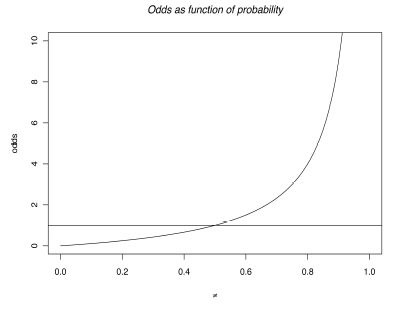
\includegraphics[width=0.9\linewidth]{odds}
\end{figure}
\end{frame}

%---------------------------------------
\begin{frame}[fragile] \frametitle{Risks and comparative parameters estimated}

The risks $\pi_1$ and $\pi_0$ are estimated by empirical incidence proportions $R_1=D_1/N_1$, and $R_0=D_0/N_0$.

\bigskip
Crude estimates of comparative parameters
\bi
\item {\bf incidence proportion difference} $\quad \text{RD} = R_1 - R_0$
\item {\bf incidence proportion ratio} $\quad \quad \quad \text{RR} = R_1/R_0$
\item {\bf incidence odds ratio}
$$\text{OR} = \frac{R_1/(1 - R_1)}{R_0/(1 - R_0)}$$
\ei

{\bf NB}. To remove {\it confounding}, the estimated must be adjusted for relevant {\it confounders}.
\end{frame}

%----------------------------------------------------------------------------------
\begin{frame}[fragile] \frametitle{Example: OS vs. PN (cont'd)}
\ \\
Crude estimates of true risk difference $\theta$, risk ratio $\phi$, and \\ odds ratio $\psi$ between OS and PN:
\begin{eqnarray*}
\RD & = & \frac{77}{350} - \frac{60}{350} = 0.22 - 0.171 = 
        + {\bf 0.049} \ (+ 4.9\%)\\
\RR & = & \frac{77/350}{60/350} = \frac{77/60}{350/350} = \frac{0.22}{0.171} = {\bf 1.283}\\
\OR & = & \frac{77/273}{60/290} = \frac{0.22/(1 - 0.22)}{0.171/(1 - 0.171)} = {\bf 1.363}
\end{eqnarray*}

PN appears more successful than OS.

Is this (a) true, (b) due to bias, or (c) due to chance?
\end{frame}


%-------------------------------------------------------------------

\begin{frame}[fragile] \frametitle{Tools for assessing precision in estimation}

(a) Difference parameters:
\bi
\item {\it standard error} of estimate SE,
\item {\it error margin} at level $c$: $\EM = z_c \times \SE$,
\item {\it confidence interval} at level $c$: $\CI = [\text{est}-\EM, \text{est}+\EM]$,
\ei

(b) Ratio parameters:
\bi
\item standard error of log-estimate SEL,
\item error factor at level $c$: $\EF = \text{exp}(z_c \times \SEL)$,
\item confidence interval at level $c$: $\CI = [\text{est}/\EF, \text{est} \times \EF]$,
\ei

where $z_c$ is an appropriate standard Gaussian quantile.
% for confidence level $c$.

{\bf NB}. These simple approximate CI formulas are based on the Wald statistics.  More accurate but complicated procedures are recommended when computationally available.
\end{frame}

%----------------------------------------------------------------------------------

\begin{frame}[fragile] \frametitle{Precision in risk difference estimation}
\ \\
Standard error of RD,  error margin at level 95\% \\($c = 0.95$, $z_c = 1.96$), and 95\% confidence interval for $\theta$:
\bes
 \SE  & = & \sqrt{ \frac{ R_1 (1- R_1) } {N_1} 
                        + \frac{ R_0 (1- R_0) } {N_0} } \\     
            & = & \sqrt{ \frac{ R_1^2 (1 - R_1 ) } {D_1} 
                 + \frac{ R_0^2 (1 - R_0 ) } {D_0} }  \\ \\
  \EM       & = & 1.96 \times \SE  \\ \\
 \CI        & = & [ \RD - \EM , \RD +  \EM ]
\ees
{\bf NB}. Standard error depends inversely on numbers of outcome cases $D_1$ and $D_0$ in the two exposure groups.
\end{frame} 

%---------------------------------------
\begin{frame}[fragile] \frametitle{Example: OS vs. PN (cont'd)}

\bes 
   \SE & = & \sqrt{ \frac{0.22 \times (1-0.22)} {350} 
                        +  \frac{0.171\times (1-0.171)} {350} } \\[20pt]
              & = & {\bf 0.030} \quad (3\ \% \mbox{-points}), \\ 
 \EM & = & 1.96 \times 0.030  =  {\bf 0.059}, 
\ees 
95 \% CI for true risk difference $\theta$:
$$ [ 0.049 - 0.059, \ 0.049 + 0.059 ]
   = [ -{\bf 0.010} , + {\bf 0.108} ] $$
   
{\it i.e.} from -1.0 to +10.8 percent points.

PN appears more successful than OS, although \\ 
the evidence is quite weak.
\end{frame} 

%----------------------------------------

\begin{frame}[fragile] \frametitle{Precision in risk ratio estimation}
\ \\
Standard error of log(RR), 95\% error factor (EF) of RR, and 95\% CI for true risk ratio $\phi$:
\bes
\SEL & = & \sqrt{ \frac{1}{D_1} + \frac{1}{D_0} - \frac{1}{N_1} - \frac{1}{N_0}} \approx \sqrt{\frac{1}{D_1} + \frac{1}{D_0}}\\
& { } & {  }\\
\EF & = & \text{exp}\{1.96 \times \SEL\}\\
& { } & {  }\\
\CI & = & [\RR/\EF, \RR \times \EF].
\ees

{\bf NB}.  Precision depends essentially on the numbers of exposed and unexposed cases, especially in a ``rare disease'' setting, where the numbers of cases are small in relation to group sizes.

\end{frame}

%---------------------------------------------------------------

\begin{frame}[fragile] \frametitle{Example: OS vs. PN (cont'd)}
\ \\
Standard error of log(RR), 95\% error factor (EF) of RR, and 95\% CI for true risk ratio $\phi$:
\bes
\SEL & = & \sqrt{ \frac{1}{73} + \frac{1}{60} - \frac{1}{350} - \frac{1}{350}}\\
     & = & {\bf 0.1547}\\
     & { } & {  }\\
\EF & = & \text{exp}\{1.96 \times 0.1547\}\\
    & = & {\bf 1.3543}\\
    & { } & {   }\\
\CI & = & [1.2833/1.3543, 1.2833 \times 1.3543]\\
    & = & [{\bf 0.9476}, {\bf 1.7380}].
\ees
\end{frame}

%------------------------------------------------------------------

\begin{frame}[fragile] \frametitle{Precision in odds ratio estimation}
\ \\
Standard error of log(OR), 95\% error factor (EF) of OR, and 95\% CI for true odds ratio $\psi$:
\bes
\SEL & = & \sqrt{ \frac{1}{D_1} + \frac{1}{D_0} + \frac{1}{C_1} + \frac{1}{C_0}}  \\
& { } & {  }\\
\EF & = & \text{exp}\{1.96 \times \SEL\}\\
& { } & {  }\\
\CI & = & [\OR/\EF, \OR \times \EF].
\ees

{\bf NB}.  Precision depends again on the numbers of exposed and unexposed cases, especially in a ``rare disease'' setting, where the numbers of cases are small in relation to group sizes.

\end{frame}

%------------------------------------------------------------------------------------

\begin{frame}[fragile] \frametitle{Example: OS vs. PN (cont'd)}
\ \\
Standard error of log(OR), 95\% error factor (EF) of OR, and 95\% CI for true odds ratio $\psi$:
\bes
\SEL & = & \sqrt{ \frac{1}{77} + \frac{1}{60} + \frac{1}{273} + \frac{1}{290}}  \\
     & = & {\bf 0.1917}\\
& { } & {  }\\
\EF & = & \text{exp}\{1.96 \times 0.1547\}\\
    & = & {\bf 1.4562}\\
& { } & {  }\\
\CI & = & [1.3632/1.4562, 1.3632 \times 1.4562]\\
    & = & [{\bf 0.9362}, {\bf 1.9851}].
\ees
\end{frame}

%--------------------------------------------------------------------

\begin{frame}[fragile] \frametitle{Estimating comparative parameters in R}
\ \\
\bi
\item A multitude of R functions in several packages are readily available for point estimation and CI calculation using either ``exact'' or/and various approximative methods.
\medskip
\item We shall here demonstrate the use of function {\tt twoby2()} in the {\tt Epi package}.  It applies the simple Wald approximations as described above, but for 
  \bi
  \item risk difference: the Newcombe method is used, and 
  \item odds ratio: the ``exact'' conditional method is also available.
  \ei
\item[ ] Hence, similar results are expected as obtained above.
\ei
\end{frame}

%------------------------------------------------------------------------

\begin{frame}[fragile] \frametitle{Use of function {\tt twoby2()}}
\bi
\item Loading the {\tt Epi package}:\\
\verb|> library(Epi)| \medskip
\item Reading the counts of the 2 x 2-table into a matrix: \\
\verb|> counts <- c(77, 273, 60, 290)| \\
\verb|> tab <- matrix( counts, nrow=2, byrow=T)|\medskip
\item Viewing the contents of the matrix/table: \\
\verb|> tab| \\
\verb|     [,1] [,2]| \\
\verb|[1,]   77  273| \\
\verb|[2,]   60  290| \medskip
\item Calling the function with {\tt tab} as its argument: \\
\verb|> twoby2(tab)|
\ei
\end{frame}

%--------------------------------------------------------------------------------

\begin{frame}[fragile] 
\frametitle{Output from {\tt twoby2()}}
\small

\begin{verbatim}
Outcome   : Col 1 
Comparing : Row 1 vs. Row 2 

      Col 1 Col 2    P(Col 1) 95% conf. interval
Row 1    77   273      0.2200    0.1797   0.2664
Row 2    60   290      0.1714    0.1355   0.2146

                                   95% conf. interval
             Relative Risk: 1.2833    0.9476   1.7380
         Sample Odds Ratio: 1.3632    0.9362   1.9851
Conditional MLE Odds Ratio: 1.3626    0.9206   2.0237
    Probability difference: 0.0486   -0.0188   0.1155

             Exact P-value: 0.1272 
        Asymptotic P-value: 0.1061 
------------------------------------------------------
\end{verbatim}
\normalsize
\end{frame}

%----------------------------------------------------------------------

\begin{frame}[fragile] 
\frametitle{Analyses based on binary regression model}

Crude estimates and CIs for the comparative parameters can also be obtained by fitting appropriate {\bf binary regression models} for the numbers $D_j$ or proportions $R_j$.

Special cases of {\bf generalized linear models} (GLM) with
\bi
\item[(i)] {\bf random part}: $D_j$ is assumed to obey the binomial distribution or {\bf family} with index $N_j$ and probability $\pi_j$, \medskip
\item[(ii)] {\bf systematic part}: {\bf linear predictor} $\eta_j = \alpha + \beta X_j$, in which $X_j = 0$ for unexposed and $X_j = 1$ for exposed, \medskip
\item[(iii)] {\bf link function}: $g(.)$ that connects the probability $\pi_j$ and the systematic part $\eta_j$ by: $$g(\pi_j) = \eta_j = \alpha + \beta X_j$$
\ei
\end{frame}

%--------------------------------------------------------------

\begin{frame}[fragile]
 \frametitle{Link functions and comparative parameters}

General model: $g(\pi_j) = \alpha + \beta X_j$ for the risks by binary $X$
\bi
\item {\bf identity} link: $g(\pi_j) = \pi_j = \alpha + \beta X_j$:\\
      $\Rightarrow \beta=\pi_1-\pi_0=\theta$, \\
      = \underline{risk difference} btw $X_j=1$ and $X_j=0$
      \medskip
\item {\bf logarithmic} link: $g(\pi_j) = log(\pi_j)$\\
$\Leftrightarrow \pi_j=\text{exp}(\alpha + \beta X_j)=e^{\alpha}e^{\beta X_j}$\\
$\Rightarrow \beta= \text{log}(\pi_1)-\text{log}(\pi_0)= \text{log}(\phi)$, \\
$\Rightarrow e^{\beta}=\phi$ = \underline{risk ratio} btw exposed and unexposed,
\medskip
\item {\bf logit} link: $g(\pi_j)=\text{log}[\pi_j/(1-\pi_j)]$
$$\Leftrightarrow \quad \pi_j=\frac{1}{1+\text{exp}\{-(\alpha + \beta X_j)\}}=\text{expit}(\alpha + \beta X_j)$$
\ei
\end{frame}

%-----------------------------------------------------------------------------------------

\begin{frame}[fragile] \frametitle{Logit model for odds ratio}
\ \\
Substituting logit function for $g(.)$ and values of $X_j$ we get
\bes
\text{log}\left(\frac{\pi_0}{1-\pi_0}\right) & = & \alpha = \text{baseline logit}\\
\text{log}\left(\frac{\pi_1}{1-\pi_1}\right) & = & \alpha + \beta.
\ees
This implies
\bes
\pi_0 & = & \frac{1}{1+\text{exp}(-\alpha)}, \quad \pi_1 = \frac{1}{1+\text{exp}\{-(\alpha+\beta)\}},\\
\beta & = & \text{log}\left\{\frac{\pi_1/(1-\pi_1)}{\pi_0/(1-\pi_0)}\right\}\\
e^{\beta} & = & \frac{\pi_1/(1-\pi_1)}{\pi_0/(1-\pi_0)} = \psi = \text{\underline{odds ratio} btw exp'd and unexp'd.}
\ees
\end{frame} 

%-----------------------------------------------------------------------------------

\begin{frame}[fragile] \frametitle{Fitting binary regression models in R}
\ \\
Function {\tt glm()}
\bi
\item estimation method: {\bf maximum likelihood} (ML),
\item computation algorithm: IWLS.
\ei

\medskip
Key arguments of {\tt glm()}:
\bi
\item model formula: {\it ``response'' $\sim$ ``expression of regressors''}
\medskip
\item {\tt weights} = group sizes $N_j$ when proportions $R_j$ are given as the response (outcome) variable,
\medskip
\item
\small {\tt family = binomial(link = 'log')}, if risk ratio,\\
      {\tt family = binomial(link = 'logit')}, if odds ratio, \\
      {\tt family = binomial(link = 'identity')}, if risk diff'ce \\
      $\qquad$ is the parameter of interest.
\normalsize      
\ei
\end{frame}

%---------------------------------------------------------------------------

\begin{frame}[fragile] \frametitle{Example: Treatment of renal calculi (cont'd)}
\ \\
Grouped data set comprises
\bi
\item two observations (one for each treatment group),\medskip
\item three variables: 
  \bi
   \item[ ]
        {\tt treat} = treatment, with values 1 = OS, 0 = PN,
   \item[ ]        
        {\tt fail} = number of failures $D_j$, 
   \item[ ]
        {\tt npat} = number of patients $N_j$,
  \ei
\item variable vectors defined:
\small
\begin{verbatim}
> treat <- c(0, 1)
> fail <- c(60, 77)
> npat <- c(350, 350)
> prop <- fail/npat
\end{verbatim}
\normalsize
\ei
\end{frame} 

%------------------------------

\begin{frame}[fragile]
 \frametitle{Estimation of risk ratio}
 
\bi
\item Defining the {\it model object}: 
\small
\begin{verbatim}
> RRmodel <- glm( prop ~ treat, 
+   family=binomial(link='log'), weights=npat)
\end{verbatim}
\normalsize
\item Estimation results extracted by function {\tt ci.lin()} in {\tt Epi}\\
(two columns of the whole output omitted for clarity)\small
\begin{verbatim}
> round( ci.lin(RRmodel, Exp=T)[, -(3:4)], 4)
            Estimate StdErr exp(Est.)   2.5%  97.5%
(Intercept)  -1.7636 0.1175    0.1714 0.1362 0.2158
treat         0.2495 0.1547    1.2833 0.9476 1.7380
\end{verbatim} 
\normalsize
\medskip
\item The estimate of $\beta$ is $\widehat\beta = 0.2495 = \text{log}(1.2833)$, and that of risk ratio $\phi$ is $\RR = \text{exp}(0.2495) = 1.2833$.\medskip
\item Estimate of $\alpha$ is 
$\widehat\alpha = -1.7636 = \text{log}(0.1714) = \text{log}(R_0)$.\medskip
\item Previous results recovered also for SEL and CI.
\ei
\end{frame}

%------------------------------------------------------------------------

\begin{frame}[fragile] \frametitle{Estimation of odds ratio}

\small
\begin{verbatim}
> ORmodel <- glm( prop ~ treat, 
       fam = binomial(link='logit'), weights=npat)
       
> round( ci.lin(ORmodel, Exp=T)[, -(3:4)], 4)
            Estimate StdErr exp(Est.)   2.5%  97.5%
(Intercept)  -1.5755 0.1418    0.2069 0.1567 0.2732
treat         0.3099 0.1917    1.3632 0.9362 1.9851
\end{verbatim}
\normalsize
\bi
\item The estimate of $\beta$ is $\widehat\beta = 0.3099 = \text{log}(1.3632)$, and the estimated $\psi$ is 
      $\text{OR} = \text{exp}(0.3099) = 1.3632$.
      \medskip
\item The estimate of $\alpha$ is $\widehat\alpha -1.5755 = \text{log}(0.2069)$, in which\\
      $0.2069 = 0.1714/(1 - 0.1714)$ is the estimated\\
      baseline odds $R_0/(1 - R_0)$.
\ei
\end{frame} 

%-----------------------------------------------------------------------------------

\begin{frame}[fragile]
 \frametitle{Estimation of risk difference}

\small
\begin{verbatim}
> RDmodel <- glm( prop ~ treat, 
    fam=binomial(link='identity'), w=npat)
    
> round( ci.lin(RDmodel), 3)
            Estimate StdErr     z     P   2.5% 97.5%
(Intercept)    0.171   0.02 8.510 0.000  0.132 0.211
treat          0.049   0.03 1.623 0.105 -0.010 0.107
\end{verbatim}
 \normalsize
\bi 
\item Again, same results obtained as with 
{\it e.g.} {\tt twoby2()},
  although CIs are here based on Wald statistic.
\medskip
\item {\bf NB}. Fitting binomial model with this link 
easily fails with more complicated models, 
      especially involving continuous variables.
\ei
\end{frame}

%----------------------------------------------------------------------------------------

\begin{frame}[fragile] \frametitle{Confounding and effect modification}
\ \\
Consider another {factor} $Z$ which is
\bi
\item also a risk factor of the outcome,
\item possibly associated with exposure $X$ in study population,
\item not a causal consequence of $X$.
\ei

$\Rightarrow$ Adjustment for possible {\it confounding} and evaluation of {\it effect modification} needed.
\end{frame} 

%----------------------------------------------------------------

\begin{frame}[fragile] \frametitle{Example: OS vs. PN (cont'd)}
\ \\
Failure of treatment depends also on initial condition
of patient, like extent and severity of disease.

Results stratified by initial diameter size of the stone:

\begin{center}
\begin{tabular}{lcrrcc}
\toprule
Size   &   Trt        & Fails  & Npats & Fail-\% & {\bf RD(\%)}\\
\midrule
$<$ 2 cm  &  OS                &         6        &  87        &        {\em 6.9}  & { } \\
 & PN                &        35        & 270        &        {\em 13.0} & {\bf $-$6.1} \\
\midrule
$\geq$ 2 cm  &  OS         &          71 &        263        & {\em 27.0} & { }  \\
  &  PN         &          25 &         80        & {\em 31.3} & 
  {\bf $-$4.3} \\
\bottomrule
\end{tabular}
\end{center}

OS seems more successful in both subgroups, even though overall PN appeared better.

{\it IS THERE A PARADOX?}
\end{frame} 

%--------------------------------------------

\begin{frame}[fragile] \frametitle{Confounding}
\ \\
Solution:
Treatment groups are not {\it comparable}
w.r.t. initial size.
Size of the stone is a {\bf confounder}
of the association between operation type
and failure risk,because it is
\bi
\item[1.] an {\it independent determinant} of outcome (failure), based on
external knowledge,
\item[2.] {\it statistically associated} with operation type in the
   study population,
\item[3.] {\it not causally affected} by operation type.
\ei

This is an instance of ``confounding by indication'':
\bi
   \item patient status
affects choice of treatment 
  \item[$\to$] {\it bias} in comparing treatments.
\ei

This bias would be best to avoid in planning: \\
$\rightarrow$
 {\it randomized allocation} of treatments!
\end{frame} 

%----------------------------------------------

\begin{frame}[fragile] \frametitle{Stratified analysis}
Stratification of cohort data with proportions 
\bi
\item[--] at each level $k$ of factor $Z$ results are summarized:
\ei
\begin{center}
\begin{tabular}{cccc}
\toprule
Exposure to &  Number of &  Number of &  Group\\
risk factor &  cases &  non-cases  &  size\\
\midrule
yes        &                $D_{1k}$ &    $C_{1k}$  &    $N_{1k}$ \\
no         &                $D_{0k}$ &    $C_{0k}$  &    $N_{0k}$ \\
\midrule    
     Total        &                $D_{\+ k}$  &  $C_{\+ k}$  &   $N_{\+ k}$ \\
\bottomrule
\end{tabular}
\end{center}

Stratum-specific incidence proportions by exposure group: 
$$ R_{1k}  = \frac{ D_{1k} }{ N_{1k} } , \qquad
   R_{0k}  = \frac{ D_{0k} }{ N_{0k} } $$
\end{frame} 

%------------------------

\begin{frame}[fragile] \frametitle{Adjusted estimation of risk difference}
\ \\
\bi
\item Let $\pi_{jk}$ be true risk in exposure group $j$ ($j=0,1)$ as to $X$
and stratum $k$ ($k=0, \dots, K$) of $Z$. Let also
$$ \theta_k = { \pi_{1k} } - { \pi_{0k} } $$
be the risk difference in stratum $k$.
\medskip
\item Many approaches to combine stratum specific results 
into one summary estimator that adjusts for confounding.

\medskip
These are all somehow {\em weighted averages} of stratum-specific
estimators.
\medskip
\item Different weighting principles:
  \bi
  \item Maximum likelihood (ML), 
  \item Mantel-Haenszel (MH) weights,
  \item Standardization either by external standard population 
  or by ``indirect'' standardization.
  \ei
\ei
\end{frame} 

%--------------------------

\begin{frame}[fragile] \frametitle{Model-based adjustment of risk difference}
\ \\
Define generalized linear model for binary outcome with
\bi
\item one binary exposure variable $X$ and 
\item
one binary stratifying factor or covariate $Z$ (easily generalized to polytomous factors).
\ei

{\it Random part}: Number of cases $D_{jk}$ in exposure group $j$ ($j=0,1$) of $X$ 
and level $k$ $(k = 0, 1)$ of $Z$ is assumed to be binomially distributed
$$D_{jk} \sim \text{Binomial}(N_{jk} ; \pi_{jk} ) , $$

\end{frame}

%-----------------------------------------------------------------

\begin{frame}[fragile] \frametitle{Model-based adjustment of risk difference (cont'd)}
\ \\
{\it Systematic part}: 
$$ \pi_{jk} = \alpha + \beta X_j +
  \gamma Z_k  , $$
where $X_j$ is 0/1-indicator as before, and
\bi \item[]
\bi
\item[]$Z_k =$ 1 for level $k=1$ of $Z$, otherwise $Z_k =$ 0,
\item[]$\alpha= \pi_{00}$ = baseline (''corner cell'') risk, 
\item[]$\gamma= \pi_{01}- \pi_{00} = \pi_{11} - \pi_{10}$,
\item[]$\beta= \pi_{10} - \pi_{00} = \theta_0$
                = $\pi_{11} - \pi_{01} = \theta_1$,
\ei
\ei
{\it How do we read this?}

\end{frame} 

%----------------------------------------------

\begin{frame}[fragile] \frametitle{Model-based adjustment of risk difference (cont'd)}
\ \\
Implications of model definition
\bi
\item the model assumes {\bf homogeneity} of true risk difference $\theta$ associated with factor $X$ (exposed vs. unexposed) across levels of $Z$: $\theta_1 = \theta_0 = \beta$,
\medskip
\item inclusion of $Z$ in the model leads to adjustment of it when estimating the ``true'' effect $\theta$ of 
      $X$,\medskip
\item $\gamma$ = risk difference between levels $1$ and 0 of $Z$; this
      is same in both exposure groups ($j=0,1$)  \newline
      $\Rightarrow$ homogeneity of the effect of $Z$ is assumed, too.
\ei
\end{frame} 

%----------------------------------------------

\begin{frame}[fragile] \frametitle{Example. Treatment of renal calculi (cont'd)}

\bi
\item Define new variable\\ 
$\quad$ {\tt size} = initial stone size (0 for ``small'', 1 for ``large'')
\medskip
\item Extended data matrix comprises four observational units (rows) and four variables (columns):
\small
\begin{verbatim}
     size   trt   fails   npats
       0      1       6      87   
       0      0      35     270
       1      1      71     263 
       1      0      25      80  
\end{verbatim}
\normalsize
\medskip
\item These may be read in as before, {\it e.g.}
\small
\begin{verbatim}
size <- c( 0, 0, 1, 1) ; trt <- c( 1, 0, 1, 0)
fails <- c( 6, 35, 71, 25)
npats <- c( 87, 270, 263, 80) 
props <- fails/npats
\end{verbatim}
\normalsize
\ei
\end{frame} 

%-----------------------------

\begin{frame}[fragile] \frametitle{Fitting model for adjusted risk difference}
 
As before, but model formula supplemented by {\tt + size}
\small
\begin{verbatim}
> RDmod2 <- glm( props ~ trt + size, 
+      fam = binomial(link='identity'), w = npats)

> round( ci.lin(RDmod2), 3)
            Estimate StdErr      z     P   2.5% 97.5%
(Intercept)    0.128  0.019  6.596 0.000  0.090 0.166
trt           -0.056  0.030 -1.888 0.059 -0.114 0.002
size           0.195  0.032  6.106 0.000  0.132 0.258
\end{verbatim} 
\normalsize
Reading the results:
\bi
\item[ ]$\ \widehat\alpha\ $ = {\bf 0.128} = $\widehat\pi_{00}$, fitted baseline risk,
\item[ ]$\ \widehat\gamma\ $ = {\bf 0.195}, RD between large and small stones,
\item[ ]$\ \widehat\beta\ $ = $-${\bf 0.0561} [$-${\bf 0.114},
 {\bf 0.002}], estimated \\ $\qquad$ common
  treatment effect $\widehat \theta$ for OS {\it vs.} PN.\\
$\quad$ = Weighted average of $\widehat \theta_0 = -0.061$ and $\widehat \theta_1 = -0.043$.
\ei

\end{frame} 

%----------------------------------------

\begin{frame}[fragile] \frametitle{Effect modification}

 \ \\ 
Homogeneity assumption -- 
true differences were put equal:
$$ \theta_k = \pi_{1k} - \pi_{0k} = \theta $$ 
across all levels $k$ of covariate $Z$.
{\it Is this realistic?}

\bigskip
{\it Example.} Is the true risk difference for treatment failure 
between OS and PN similar for small and big stones?

Empirical differences of failure proportions were
\bes \text{small stones}: \widehat\theta_0 & = & 0.069 - 0.130 = {\bf -0.061} \\
     \text{large stones}: \widehat\theta_1 & = & 0.270 - 0.313 = {\bf -0.043}
\ees
Is the contrast $-0.043 - (-0.061) = 0.018$
between these differences due to chance only, or
is there essential \\ {\bf effect modification} present?
\end{frame} 

%----------------------------------------

\begin{frame}[fragile]
\frametitle{Modelling modification of risk difference}
\ \\
The random part is the same, but the systematic part is
\begin{center}
$ \pi_{jk} = \alpha + \beta X_j +
  \gamma Z_k + \tau U_{jk} . $ 
  \end{center}
\bi 
\item[]$U_{jk}= X_j \times Z_k$, product of values of $X$ and $Z$,
\item[]$\alpha=  \pi_{00}$ = baseline (''corner cell'') risk, 
\item[]$\beta= \pi_{10} - \pi_{00} = \theta_0, \qquad
                \gamma = \pi_{01}- \pi_{00}$,
\item[]$\tau= \theta_1 - \theta_0$ 
        = $(\pi_{11} - \pi_{01}) - ( \pi_{10} - \pi_{00})$,\\
        $\qquad$ {\bf interaction parameter}
\ei
$\tau$ describes, how much greater is the risk difference 
between levels 1 and 0 of risk factor $X$ among those at
level 1 of factor $Z$ than in those at level 0.
\end{frame} 

%-----------------------------------------

\begin{frame}[fragile] \frametitle{Fitting model with modification}
\bi
\item
Generation of an interaction of {\bf product term}:
\bi
\item[ ] \verb|> trtsize = size*treat|
\ei
\item
Expanded and rearranged data matrix: \small
\begin{verbatim}
 fails   npats       size       trt    trtsize
   35     270          0         0         0
    6      87          0         1         0
   25      80          1         0         0
   71     263          1         1         1
\end{verbatim} \normalsize
\item
Fitting the model including the product term: 

\medskip
\verb|> RDmod3 <- glm( props ~ trt + size + trtsize,|
\verb|+     fam = binòmial(link='identity', w = npats)|
\ei
\end{frame} 

%-----------------------------------------

\begin{frame}[fragile] \frametitle{Fitting model with modification (cont'd)}
\ \\
Results and interpretation:
\small
\begin{verbatim}
> round( ci.lin(RDmod3)[ , -(3:4)], 4)
            Estimate StdErr    2.5%  97.5%
(Intercept)   0.1296 0.0204  0.0896 0.1697
trt          -0.0607 0.0340 -0.1273 0.0060
size          0.1829 0.0557  0.0737 0.2921
trtsize       0.0181 0.0678 -0.1147 0.1509
\end{verbatim}
\normalsize
\bi
\item $\widehat \beta = -0.061 = \widehat \theta_0 =$ RD for OS {\it vs.} PN in small stones,
\item $\widehat \gamma = -0.183 =$ RD btw large and small stones for OS.
\item estimate [95 \% CI] of the interaction parameter:
$$\widehat \tau = {\bf 0.0181 [-0.115, 0.151]}$$
\item[{ }] $\Rightarrow$ no evidence for essential modification of risk difference.
\ei
\end{frame} 
%------------------------------------------

\begin{frame}[fragile] \frametitle{Interpretation}
\ \\
This model is {\it saturated}: It has as many 
coefficients as there are observations. Hence
\bi
\item residual df = 0,
\item fitted cell probabilities = observed proportions:
  \bi 
 \item[]$\widehat\pi_{00}$  = $0.130$, 
 \item[]$\widehat\pi_{10}$  = $0.130 - 0.061 = 0.069$,
 \item[]$\widehat\pi_{01}$  = $0.130 + 0.183 = 0.313$,
 \item[]$\widehat\pi_{11}$  = $0.130 - 0.061 + 0.183 + 0.018$ 
  = 0.027
  \ei
\item residual $X^2$ and deviance are both 0.
\ei
\end{frame} 
%-------------------------------------------

\begin{frame}[fragile] \frametitle{Final comments}

\bi
\item When risk ratio $\phi$ or odds ratio $\psi$ is the parameter of interest, adjustment for confounding and evaluation of modification can be done by fitting an analogous binomial GLM with relevant link function.

\item Modelling can easily be extended to cover one or more polytomous and/or continuous covariates.  Flexible functional forms may be specified to describe the effects of the latter type of variables.

\item Binomial models are not limited to grouped data but may be fitted on individual data with binary outcomes, too.

\item With more complicated models, especially involving continuous variables, the identity  link (sometimes log link, too) violates the basic range restriction:\\
outcome probabilities $\pi$ must remain within 0 and 1. 
\ei
\end{frame}

%-----------------------------------------------------------------



\end{document}

